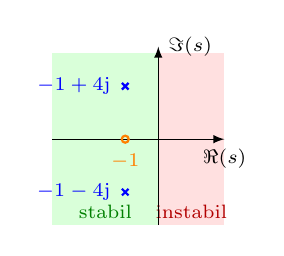
\begin{tikzpicture}[>=latex, font=\scriptsize, scale=0.42]
  % Halbebenen: links stabil, rechts instabil
  \fill[green!15] (-3.2,-2.6) rectangle (0,2.6);
  \fill[red!12]   (0,-2.6)    rectangle (2,2.6);
  \node[green!50!black] at (-1.6,-2.2) {stabil};
  \node[red!70!black] at (1,-2.2) {instabil};
  \draw[-latex] (-3.2,0) -- (2,0) node[below] {$\Re(s)$};
  \draw[-latex] (0,-2.6) -- (0,2.8) node[right] {$\Im(s)$};
  % Nullstelle (Kreis)
  \draw[thick, orange] (-1,0) circle (3pt);
  \node[orange, below] at (-1,-0.15) {$-1$};
  % Pole (Kreuze)
  \foreach \y in {1.6,-1.6}
    \draw[thick, blue] (-1.1,\y-0.1) -- (-0.9,\y+0.1)
                       (-1.1,\y+0.1) -- (-0.9,\y-0.1);
  \node[blue, left] at (-1.15,1.6)  {$-1+4\mathrm{j}$};
  \node[blue, left] at (-1.15,-1.6) {$-1-4\mathrm{j}$};
\end{tikzpicture}
